%! TEX program = xelatex
\PassOptionsToPackage{dvipsnames,table}{xcolor}
% \documentclass[draft,compress]{beamer}
\documentclass[compress]{beamer}

\usepackage{kotex}
\usepackage{minted}
\usepackage[export]{adjustbox}

\usepackage[usebold,usecolor,color=blue]{xmph}

% \usepackage{kotex-logo}

% \usepackage{tikz}
% \usetikzlibrary{patterns,decorations.pathmorphing}

\vfuzz=30pt
\hfuzz=5pt

%%%%%%%%%%%%%%%%%%%%%
%  Beamer Settings  %
%%%%%%%%%%%%%%%%%%%%%
\usetheme[
  numbering=fraction,
  subsectionpage=progressbar
]{metropolis}
\usecolortheme{rose}
\useoutertheme[subsection=false]{miniframes}

\setbeamertemplate{itemize item}[square]
\setbeamertemplate{itemize subitem}[triangle]
\setbeamertemplate{itemize subsubitem}[circle]

% \usepackage{pgfpages}
% \setbeameroption{show notes on second screen}

% A workaround to make miniframes circles clickable with XeTeX
% See https://tex.stackexchange.com/a/369327
\setbeamertemplate{mini frame in current section}{%
  \visible<0>{\resizebox{0.1cm}{0.1cm}{o}}\kern-0.1cm%
  \begin{pgfpicture}{0pt}{0pt}{0.1cm}{0.1cm}
    \pgfpathcircle{\pgfpoint{0.05cm}{0.05cm}}{0.05cm}
    \pgfusepath{stroke}
  \end{pgfpicture}%
}
\setbeamertemplate{mini frame in current subsection}{%
  \visible<0>{\resizebox{0.1cm}{0.1cm}{o}}\kern-0.1cm%
  \begin{pgfpicture}{0pt}{0pt}{0.1cm}{0.1cm}
    \pgfpathcircle{\pgfpoint{0.05cm}{0.05cm}}{0.05cm}
    \pgfusepath{stroke}
  \end{pgfpicture}%
}

%%%%%%%%%%%%%%%%%%%
%  Font Settings  %
%%%%%%%%%%%%%%%%%%%
\usepackage[factor=500]{microtype}

\usefonttheme{professionalfonts} % required for mathspec
\usepackage{mathspec}

\setmathsfont(Digits)[%
  Numbers={Lining, Proportional}
]{Fira Sans}
\setsansfont[%
  BoldFont={Fira Sans SemiBold},
  Numbers={OldStyle}
]{Fira Sans}
\setsanshangulfont{Noto Sans CJK KR}[%
  AutoFakeSlant=0.18,
  FontFace={m}{up}{Font=*}
]

\newfontfamily\NotoSansMonoExtraCondensed{Noto Sans Mono ExtraCondensed}
\RenewDocumentCommand\UrlFont{}{\NotoSansMonoExtraCondensed}
\NewDocumentCommand\textct{m}{{\NotoSansMonoExtraCondensed#1}}

\usepackage{contour}
\contourlength{1pt}

%%%%%%%%%%%%%%%%%%%%%
%  Minted Settings  %
%%%%%%%%%%%%%%%%%%%%%
\renewcommand\theFancyVerbLine{\textsf{\tiny\arabic{FancyVerbLine}}}
\newminted{latex}{
  escapeinside=||,
  autogobble,
  linenos,
  breaklines,
  numbersep=5pt,
  frame=single,
  fontsize=\footnotesize}
\newmintinline[ltxverb]{latex}{fontsize=\footnotesize}
\NewDocumentCommand\inputltx{m}{%
  \inputminted[
    escapeinside=||,
    autogobble,
    linenos,
    breaklines,
    numbersep=5pt,
    frame=single,
    fontsize=\footnotesize
  ]{latex}{#1}}


%%%%%%%%%%%%%%%%%%%%%%%
% Custom Settings  %
%%%%%%%%%%%%%%%%%%%%%%%
\NewDocumentCommand\beamer{}{\textsc{beamer}}
\NewDocumentCommand\tpc{}{\!\textperiodcentered\!}
\NewDocumentCommand\tat{}{\textasciitilde}
\NewDocumentCommand\tla{}{\textleftarrow}
\NewDocumentCommand\tra{}{\textrightarrow}
\NewDocumentCommand\tua{}{\textuparrow}
\NewDocumentCommand\tda{}{\textdownarrow}
\NewDocumentCommand\tbs{}{\textbackslash}
\NewDocumentCommand\vpad{}{\vspace{1em}}

\newcommand*{\numberofpages}[1]{%
  \the\XeTeXpdfpagecount"#1"%
}

\newcommand\seefile[1]{%
  {\tiny 실습자료: \texttt{#1}}%
}

% https://tex.stackexchange.com/a/174818
% adapted from doc.dtx
\providecommand\meta[1]{\textlangle{\itshape #1\/}\textrangle}
% directly taken from ltxdoc.dtx
\providecommand\marg[1]{%
  {\ttfamily\char`\{}\meta{#1}{\ttfamily\char`\}}}
\providecommand\oarg[1]{%
  {\ttfamily[}\meta{#1}{\ttfamily]}}
% directly taken from listings.dtx (lstdoc.sty)
\definecolor{darkgreen}{rgb}{0,0.5,0}
\def\rstyle{\color{darkgreen}}
% adapted from listings.dtx (lstdoc.sty)
\providecommand\rcmdname[1]{\texttt{\rstyle\string#1}}


%%%%%%%%%%%%%%%%%%%%%%%
%  Document Settings  %
%%%%%%%%%%%%%%%%%%%%%%%
\title{The ``key-value'' structure in \LaTeX}
\subtitle{Live Coding}
\author{이재호}
\institute{서울대학교 전기\tpc{}정보공학부\,/\,KTUG}
\date{2021년 11월 27일}

%%%%%%%%%%%%%%
%  Document  %
%%%%%%%%%%%%%%
\begin{document}
% \RenewDocumentCommand\pause{o}{}

\maketitle

\begin{frame}[fragile=singleslide]{\LaTeX{} commands}
  \seefile{latex-commands.tex}

  \rcmdname\newcommand\marg{name}\oarg{\# of args}\oarg{first}\marg{code}

  \begin{latexcode}
    \newcommand{\N}{\mathbb{N}}
    \newcommand{\Z}{\mathbb{Z}}
    \newcommand{\R}{\mathbb{R}}
    \newcommand{\C}{\mathbb{C}}
    \newcommand{\nset}[1]{\mathbb{#1}}
    \newcommand{\ndim}[2][3]{\mathbb{#2}^{#1}}
    % ...
    $\Z, \nset{B}, \ndim{R}, \ndim[2]{C}$
  \end{latexcode}
  \newcommand{\Z}{\mathbb{Z}}
  \newcommand{\nset}[1]{\mathbb{#1}}
  \newcommand{\ndim}[2][3]{\mathbb{#2}^{#1}}
  {\huge
    \begin{equation*}
      \Z, \nset{B}, \ndim{R}, \ndim[2]{C}
    \end{equation*}
  }
\end{frame}

\begin{frame}[fragile=singleslide]{\TeX{} commands}
  \seefile{tex-commands.tex}

  \rcmdname\def\rcmdname\name\meta{param text}\marg{code}

  \begin{latexcode}
    \def\N{\mathbb{N}}
    \def\Z{\mathbb{Z}}
    \def\R{\mathbb{R}}
    \def\C{\mathbb{C}}
    \def\nset#1{\mathbb{#1}}
    \def\ndim[#1]#2{\mathbb{#2}^{#1}}
    % ...
    $\Z, \nset{B}, \ndim[3]{R}, \ndim[2]{C}$
  \end{latexcode}
  {\huge
    \def\N{\mathbb{N}}
    \def\Z{\mathbb{Z}}
    \def\R{\mathbb{R}}
    \def\C{\mathbb{C}}
    \def\nset#1{\mathbb{#1}}
    \def\ndim[#1]#2{\mathbb{#2}^{#1}}
    \begin{equation*}
      \Z, \nset{B}, \ndim[3]{R}, \ndim[2]{C}
    \end{equation*}
  }
  {\tiny
    - 사실 전의 \verb/\newcommand/에 *을 붙여야(\verb/\newcommand*/), \verb/\def/처럼 한 문단 이상 인자를 받지 않음.
  }
\end{frame}

\begin{frame}[fragile=singleslide]{Key-value?}
  본 슬라이드의 preamble에서\dots
  \begin{latexcode}
    %%%%%%%%%%%%%%%%%%%%%
    %  Beamer Settings  %
    %%%%%%%%%%%%%%%%%%%%%
    \usetheme[
      numbering=fraction,
      subsectionpage=progressbar
    ]{metropolis}
    \usecolortheme{rose}
    \useoutertheme[subsection=false]{miniframes}
  \end{latexcode}

  \note{
    Key-value 입력을 통해 좀 더 유연한 인터페이스를 제공할 수 있음.
    여러 언어에서 서로 다른 이름으로 불리우는데, 파이썬의 딕셔너리, C++이나 자바의 맵, 연관 배열 등등에 대응하는 자료 구조.
    LaTeX2e까지에서 언어 차원의 지원이 없음.
  }
\end{frame}

\begin{frame}[fragile=singleslide]{Key-value?}
  \begin{center}
    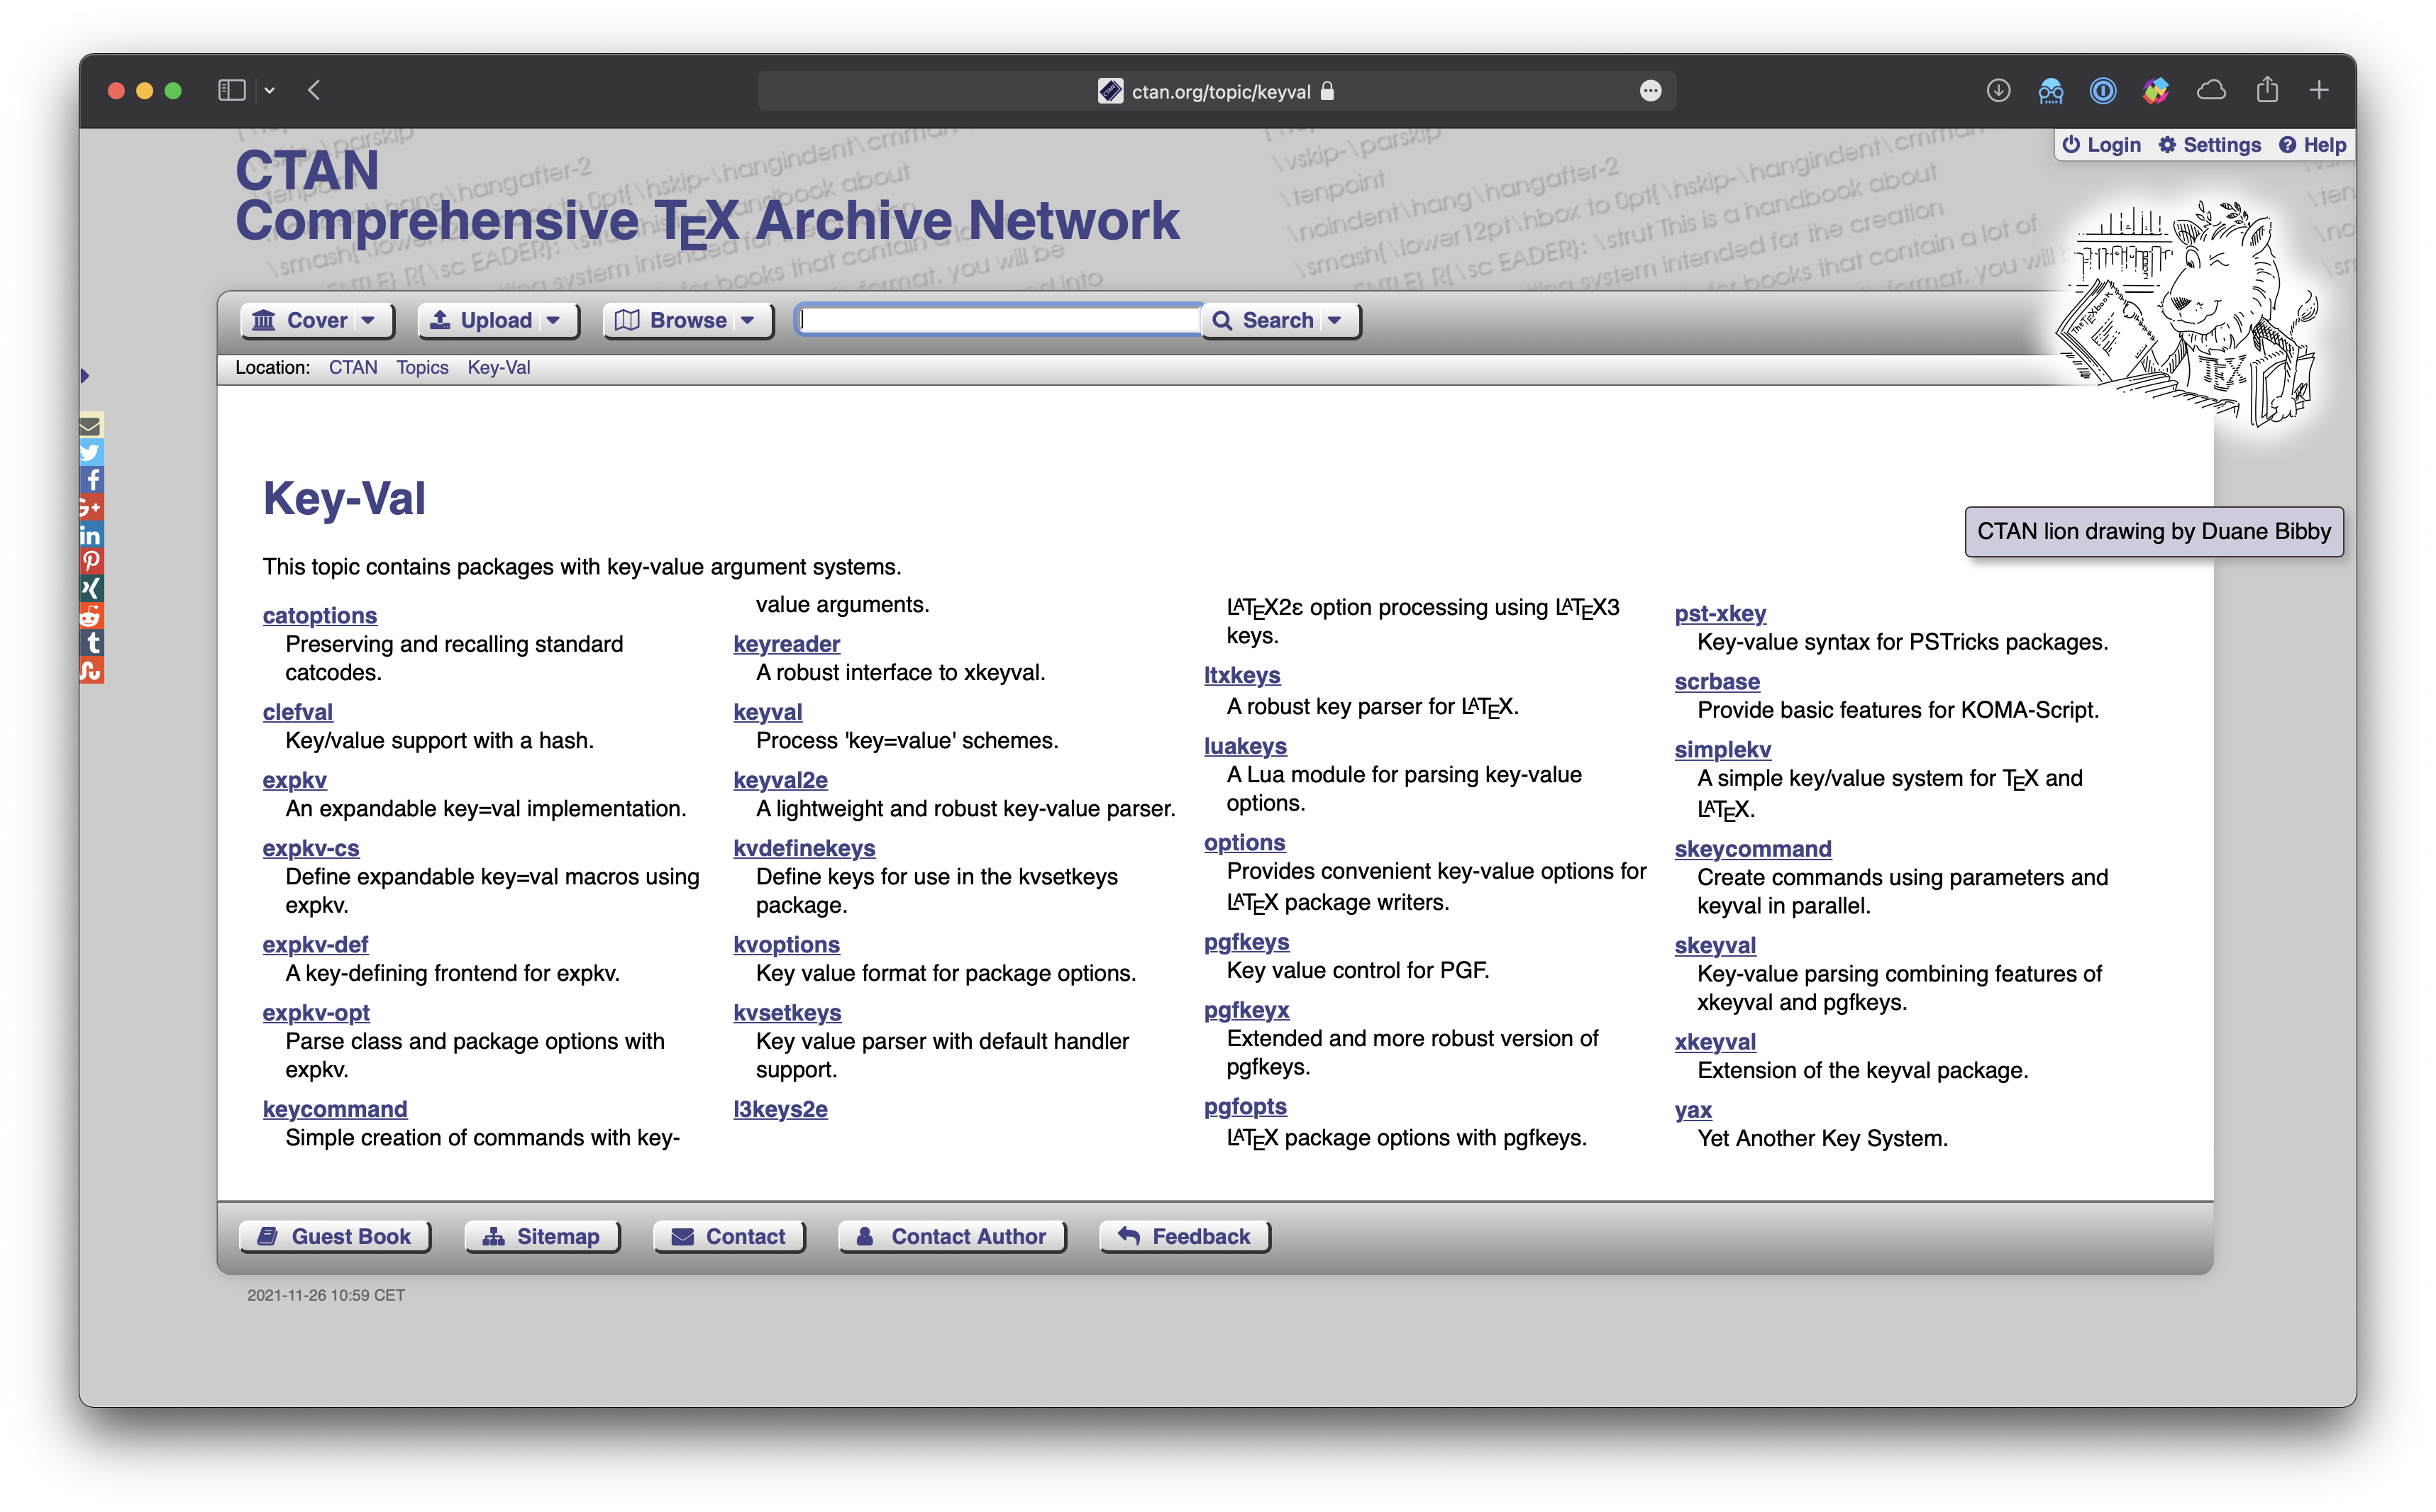
\includegraphics[width=0.9\textwidth]{figures/keyval-packages}
    \url{https://ctan.org/topic/keyval}
  \end{center}
\end{frame}

\begin{frame}[fragile=singleslide]{History}
  \begin{itemize}
    \item \textsl{keyval} (Charlisle, '99)
    \item \textsl{xkeyval} (Adriaens, '08)
    \item \textsl{kvoptions} (Oberdiek, '09)
    \item \textsl{kvsetkeys} (Oberdiek, '09)
    \item \textsl{keycommand} (Chervet, '09)
    \item \textsl{pgfkeys} (Tantau, '08)
    \item \dots
  \end{itemize}
  \note{
    \LaTeX2\varepsilon 때부터 pstricks 등의 패키지는 named argument interface를 갖춤.
    \LaTeX\ 개발자들은 인터페이스를 성급히 추가하기 보다는 기존 \LaTeX 2.09 까지 쓰인 방식을 통합하고자 함.
    아무튼 graphicx 등의 패키지는 keyval과 같은 패키지를 직접 구현하여 사용.
  }
\end{frame}

\begin{frame}[fragile=singleslide]{keyval에서 키 정의하기}
  \seefile{keyval-tutorial.tex}
  \begin{latexcode}
    % 매크로에 값 저장하기
    \define@key{fam}{name}{\def\fam@name{#1}}
    % 초기값 설정하기
    \def\fam@name{\TeX}
    \define@key{fam}{name}{%
      \def\fam@name{#1}%
    }
    % 기본값 설정하기 (!= 초기값)
    \define@key{fam}{name}[unknown]{%
      \def\fam@name{#1}%
    }
  \end{latexcode}
  기본값을 지정하면 \ltxverb/\setkeys{fam}{key}/가 \ltxverb/\setkeys{fam}{key=default}/와 동일한 효과.
\end{frame}

\begin{frame}[fragile=singleslide]{keyval에서 키 지정하기}
  \seefile{keyval-tutorial.tex}
  \begin{latexcode}
    \newcommand{\hello}{Hello, \fam@name!}
    % ...
    \hello
    \setkeys{fam}{name}
    \hello
    \setkeys{fam}{name = \LaTeX}
    \hello
  \end{latexcode}
  기본값을 설정한다고 초기값이 되는 것이 아님에 유의.
\end{frame}

\begin{frame}[fragile=singleslide]{kvoptions의 옵션 정의}
  \seefile{kvoptions-tutorial.tex, kvsample.sty}
  \begin{latexcode}
    % kvsample.sty
    \SetupKeyvalOptions{
      family=kvsample,
      prefix=kvsample@
    }
    \DeclareBoolOption{active}
    % 상호배타적인 옵션 정의
    \DeclareBoolOption{final}
    \DeclareComplementaryOption{draft}{final}
    % keyval에서 초기값 설정하기에 대응
    \DeclareStringOption[initial]{key}
    % 모든 옵션들을 처리
    \ProcessKeyvalOptions{kvsample}
    % kvoptions-tutorial.tex
    \usepackage[draft=false,active,key={val 1}]{kvsample}
  \end{latexcode}
\end{frame}

\begin{frame}[fragile=singleslide]{kvoptions의 사용}
  \seefile{kvoptions-tutorial.tex, kvsample.sty}
  \begin{latexcode}
    % kvoptions-tutorial.tex
    % 사실은 kvsample.sty에서만 써야하는 것들이지만...
    \ifkvsample@active
      {Active}
    \else
      {Inactive}
    \fi
    \ifkvsample@final
      {Final}
    \else
      {Draft}
    \fi
    Key stored: \kvsample@key
  \end{latexcode}
\end{frame}

\begin{frame}[fragile=singleslide]{kvoptions를 사용한 실례}
  \seefile{xmph-kvoptions.sty}

  \textit{Implementing key--value input: An introduction} (Wright \& Feuers\"anger, '09)
  \begin{latexcode}
    \usepackage[
      active,
      usebold,
      usecolor,
      color=blue,
    ]{xmph}
    % ...
    \xmph{a+b=c}
  \end{latexcode}
  \begin{center}
    \xmph{a+b=c}
  \end{center}
\end{frame}

\begin{frame}[fragile=singleslide]{pgfkeys의 특징}
  \begin{itemize}
    \item 키를 정의할 때도 key-value 시스템을 사용하여 편리함.
    \item 키를 정의할 때와 설정할 때 둘 다 같은 명령어를 사용.
    \item 트리 형태의 key-value 구조를 사용.
    \item `키 핸들러'라는 접미어를 사용:
      \begin{latexcode}
        \pgfkeys{/path/key/.code={#1}}
      \end{latexcode}
      와 같이 정의 후
      \begin{latexcode}
        \pgfkeys{/path/key=value}
      \end{latexcode}
      와 같이 사용하면 그대로 `value'를 출력.
    \item 이러한 특징들은 \textsl{l3keys}에서 계승.
      \begin{itemize}
        \item 다만 \textsl{l3keys}에서는 키를 정의하고 설정할 때 다른 매크로를 사용.
      \end{itemize}
  \end{itemize}
\end{frame}

\begin{frame}[fragile=singleslide]{pgfkeys의 사용}
  \seefile{xmph-pgfkeys.sty}

  \begin{latexcode*}{fontsize=\tiny}
    \newif\ifxmph@useitalic
    \newif\ifxmph@usebold
    \newif\ifxmph@usecolour
    \pgfkeys{
      /xmph/.cd,
      useitalic/.is if = xmph@useitalic,
      usebold/.is if = xmph@usebold,
      usecolour/.is if = xmph@usecolour,
      usecolor/.is if = xmph@usecolour,
      useitalic/.default = true,
      usebold/.default = true,
      usecolour/.default = true,
      usecolor/.style = {usecolour=#1},
      colour/.store in = \xmph@colour,
      color/.style = {colour=#1},
      inactive/.code = {%
        \PackageInfo{xmph}{Package inactive}
        \let\xmph\emph}}
    \pgfkeys{
      /xmph/.cd,
      useitalic,
      colour = red}
    \ProcessPgfOptions*
  \end{latexcode*}
\end{frame}

\begin{frame}[fragile=singleslide]{Expl3 live coding session}
  실습자료: \texttt{l3keys-tutorial.tex}, \texttt{textstats-*.tex}, \texttt{textstats.sty}
\end{frame}

\end{document}
